
\documentclass[conference]{IEEEtran}
\IEEEoverridecommandlockouts
% The preceding line is only needed to identify funding in the first footnote. If that is unneeded, please comment it out.
\usepackage{cite}
\usepackage{amsmath,amssymb,amsfonts}
\usepackage{algorithmic}
\usepackage{graphicx} 
\usepackage{array}   
\usepackage{multirow} 
\usepackage{textcomp}
\usepackage{amsmath}
\usepackage{xcolor}
\usepackage{blindtext}
\usepackage{hyperref}
\usepackage{multirow}
\usepackage{float}
\usepackage{stfloats}
\usepackage{longtable}
\usepackage{booktabs}
\usepackage{pdflscape} % For landscape pages
% \usepackage{caption}
\raggedbottom


% --- Begin Arabic Support Additions ---
\usepackage[english]{babel}
\usepackage{arabtex}
\usepackage{utf8}
\setcode{utf8}     
% --- End Arabic Support Additions ---

\usepackage [autostyle, english = american]{csquotes}
\MakeOuterQuote{"}

% Define a custom command for formatting Arabic text
\newcommand{\artext}[1]{%
  {\fontsize{8pt}{11pt}\selectfont \raisebox{0pt}[0pt][0pt]{\RL{#1}}}%
}


\def\BibTeX{{\rm B\kern-.05em{\sc i\kern-.025em b}\kern-.08em
    T\kern-.1667em\lower.7ex\hbox{E}\kern-.125emX}}

\makeatletter
\newcommand{\linebreakand}{%
  \end{@IEEEauthorhalign}
  \hfill\mbox{}\par
  \mbox{}\hfill\begin{@IEEEauthorhalign}
}





\begin{document}

\title{From Script to Digital: A Deep Learning Approach to Arabic Handwriting Recognition}

\author{
    \IEEEauthorblockN{Hamza Ahmed Abushahla\textsuperscript{*}}
    \IEEEauthorblockA{\textit{Department of Computer Science and Engineering} \\
    \textit{American University of Sharjah}\\
    Sharjah, United Arab Emirates \\
    b00090279@aus.edu}
    %
    \and
    %
    \IEEEauthorblockN{Ariel Justine Navarro Panopio\textsuperscript{*}}
    \IEEEauthorblockA{\textit{Department of Computer Science and Engineering} \\
    \textit{American University of Sharjah}\\
    Sharjah, United Arab Emirates \\
    b00088568@aus.edu}
    %
    \linebreakand
    %
    \IEEEauthorblockN{Layth Al-Khairulla\textsuperscript{*}}
    \IEEEauthorblockA{\textit{Department of Computer Science and Engineering} \\
    \textit{American University of Sharjah}\\
    Sharjah, United Arab Emirates \\
    b00087225@aus.edu} %test
    %
    \and
    %
    \IEEEauthorblockN{Alex Aklson\textsuperscript{†}}
    \IEEEauthorblockA{\textit{Department of Computer Science and Engineering} \\
    \textit{American University of Sharjah}\\
    Sharjah, United Arab Emirates \\
    aaklson@aus.edu}
    %
    \thanks{\textsuperscript{*}These authors contributed equally to this work.}
        \thanks{\textsuperscript{†}Author to whom correspondence should be addressed.}
}

\maketitle

\begin{abstract}
Handwritten Text Recognition (HTR) for Arabic script is crucial for enabling digital accessibility and automating the conversion of handwritten documents into searchable digital formats. The cursive nature of Arabic script, with its positional letter shapes and diacritical marks, presents significant challenges that require specialized recognition systems. These challenges are compounded by the variability in handwriting styles and the limitations of techniques developed for other languages.
In this study, we leverage the KHATT dataset to develop an end-to-end deep learning-based HTR system. Our approach effectively addresses the complexities of Arabic cursive handwriting using a segmentation-based model. This work demonstrates the potential of deep learning in advancing Arabic HTR, enabling the digitization of both contemporary and historical texts and supporting broader applications in cultural preservation and digital workflows.
\end{abstract}

% \vspace{-10pt}

\begin{IEEEkeywords}
Arabic Handwriting Recognition, KHATT Dataset, Arabic Handwriting, Optical Character Recognition, Deep Learning, Cursive Text Recognition
\end{IEEEkeywords}

\section{Introduction}

The Arabic language is the official language of 24 sovereign countries and is spoken by over 400 million people worldwide \cite{saeed2024muharaf}. It is also one of the six official working languages of the United Nations (UN), reflecting its international importance. Beyond its widespread use, Arabic holds profound cultural, literary, and religious significance, serving as a cornerstone of the heritage of Arab and Muslim communities globally \cite{ayuba2013}. This extensive reach emphasizes the importance of developing accurate Arabic handwritten text recognition (HTR) systems, which have diverse applications in educational, governmental, and cultural preservation contexts \cite{mutawa2024machine}. For instance, the ability to accurately convert both historical and contemporary handwritten Arabic documents into digital text is vital for the digitization of archives, streamlining administrative processes, and supporting large-scale data analysis efforts.

\begin{figure}[t]
  \centering
  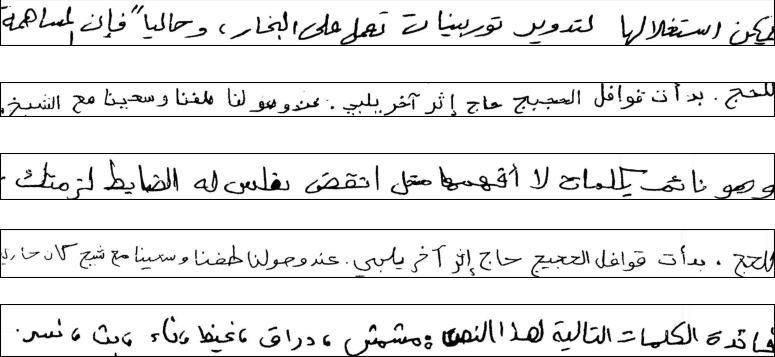
\includegraphics[width=0.9\linewidth]{Figs/fig1.png}
  \caption{Sample line images from the KHATT dataset \cite{mahmoud2014khatt}.}
  \label{fig:engagement_examples}
\end{figure}

In particular, the automated recognition and digitization of Arabic cursive handwriting present unique challenges due to the inherent complexities of the script. For one, Arabic is written from right to left, with letters assuming different shapes based on their positional context within words. In addition, diacritical marks, known as "\artext{حركات}" (harakat), and other special symbols such as the "\artext{همزة}" (hamzah) further complicate the digitization process, as many letters share identical base shapes but are distinguished by one or more dots placed above or below the character \cite{el1990arabic}. These characteristics, combined with the variability in individual handwriting styles, make the task of accurately recognizing and digitizing Arabic handwriting particularly demanding. Furthermore, because of these unique challenges, techniques developed for recognizing handwriting in other languages, such as Latin-based scripts, cannot be directly applied to Arabic, necessitating tailored approaches and specialized models \cite{alrobah2022arabic}.

Traditional Arabic HTR systems have predominantly relied on shallow learning techniques \cite{mutawa2024machine}. These methods typically involve handcrafted feature extraction processes that are sensitive to noise and degradation, limiting their effectiveness and scalability \cite{parvez2013offline}. Furthermore, most existing systems adopt a segmentation-based approach, requiring the segmentation of words into individual characters before recognition. This segmentation process is particularly challenging for Arabic due to the cursive connections between letters and the presence of similar character shapes, making it difficult to accurately isolate each character \cite{faizullah2023survey, mezghani2023recent}. In contrast, segmentation-free models (holistic approaches) recognize words as whole-word images without any segmentation processes, which can be more effective for specific applications with limited vocabularies \cite{alkhateeb2009component, nashwan2017holistic}.

Over the past decade, significant advancements in deep learning have revolutionized the field of HTR. Convolutional Neural Networks (CNNs) have emerged as the foundation of modern HTR systems due to their ability to extract complex spatial features, making them particularly effective for cursive scripts like Arabic \cite{mosbah2024adocrnet, alrobah2022arabic, altwaijry2021arabic}. Combined with Bidirectional Long Short-Term Memory (BiLSTM) networks and Connectionist Temporal Classification (CTC), deep learning models can effectively handle sequence modeling for continuous text recognition \cite{ahmad2020deep, aabed2024end, mosbah2024adocrnet,mutawa2024machine}. More recently, Transformers and attention-based models have introduced new paradigms \cite{wang2020decoupled, li2023trocr, bhunia2021metahtr}, enabling HTR systems to focus on specific regions of an image and capture long-range dependencies. These advances have significantly improved accuracy and generalizability, particularly for complex and diverse handwriting styles. Additionally, the integration of language models during post-processing has further improved prediction accuracy by leveraging contextual language information \cite{mutawa2024machine}.

To advance the development of robust HTR systems for Arabic, leveraging comprehensive and diverse datasets is paramount. While historical datasets like Muharaf \cite{saeed2024muharaf} have been valuable for analyzing historical manuscripts, there is a growing need to focus on contemporary datasets to achieve broader applicability. One such benchmark dataset is the KHATT \cite{mahmoud2012khatt,mahmoud2014khatt} dataset, which was developed by King Fahd University of Petroleum and Minerals (KFUPM) in Saudi Arabia. KHATT, an acronym for \textbf{K}FUPM \textbf{H}andwritten \textbf{A}rabic Tex\textbf{T}, also derives its name from the Arabic word (\artext{خط}), meaning ‘handwriting.’ This dataset consists of 4,000 handwritten paragraphs contributed by 1,000 writers, with each individual providing six paragraphs. The contributors reflect diverse demographics, including participants from countries such as Saudi Arabia, Morocco, the USA, Palestine, Kuwait, Egypt, Tunisia, and Yemen, representing a wide range of age groups, educational backgrounds, and both genders.

KHATT includes scanned images of handwritten text along with corresponding ground truth annotations, making it a vital resource for training and evaluating handwriting recognition systems. Its diversity in writing styles and demographics makes it especially suitable for developing generalized HTR systems that can handle the complexities of Arabic handwriting across various contexts. 


This study presents a segmentation-based HTR model utilizing advanced deep learning techniques to achieve high accuracy in Arabic handwriting recognition. The proposed system employs ResNet as a backbone for feature extraction, followed by a BiLSTM-CTC architecture for sequence modeling. To further enhance performance, a language model is incorporated during the post-processing phase, improving prediction accuracy by leveraging contextual information. In general, our contributions can be summarized as follows:


\begin{itemize}
    \item We develop a CNN-based deep learning approach combined with BiLSTM-CTC and a language model to accurately recognize Arabic handwritten text.
    \item We design a robust preprocessing pipeline to address handwriting variability and optimize input data for recognition.
    \item We rigorously evaluate our system using the KHATT dataset, demonstrating its effectiveness across diverse handwriting styles.
\end{itemize}

The remainder of this paper is organized as follows: Section 2 provides the background, including an overview of HTR, the unique characteristics of Arabic handwriting, and essential terminology. Section 3 reviews related work, covering traditional methods, advancements in deep learning, and the importance of datasets in Arabic handwriting recognition. Section 4 outlines our methodology, detailing the proposed solution, algorithms, and techniques used to address the problem. Section 5 presents the results and evaluation, discussing the findings and their implications. Finally, Section 6 concludes the study by summarizing key contributions, addressing limitations, and proposing directions for future research.


\section{Background}
%anything here?











\subsection{Handwritten Text Recognition}

\subsubsection{Introduction to OCR and the Transition to HTR}
Optical Character Recognition (OCR) laid the foundation for modern text recognition systems by enabling the automated extraction of text from printed documents. This field gained momentum in the 1990s \cite{parvez2013offline}, with early neural network models like LeNet \cite{lecun1998gradient} showcasing significant promise in character classification tasks. While OCR systems excelled at recognizing machine-printed text, handwritten text recognition (HTR) introduced additional complexities, such as variable writing styles, uneven spacing, and cursive connections. These challenges necessitated more advanced methodologies, evolving OCR into HTR to address the variability inherent in handwriting.


\subsubsection{Levels of HTR}

HTR systems tackle text recognition at different levels of granularity, beginning with character-level recognition. This approach involves recognizing isolated characters, often requiring segmentation of the text. While effective for non-cursive scripts or logographic languages like Japanese \cite{clanuwat2019kuronet} and Chinese \cite{jaderberg2015spatial}, character-level recognition struggles with cursive languages like Arabic, where the shapes of letters depend on their position and surrounding context.

To overcome these limitations, word-level recognition transcribes individual handwritten words as single units, reducing the dependency on character segmentation and improving accuracy for cursive scripts \cite{bhunia2019handwriting}. More advanced techniques have focused on line-level recognition, where entire lines of text, including spaces, are transcribed. Line-level HTR can either rely on pre-segmented input or integrate segmentation and recognition into a unified framework. Line-level recognition introduces challenges related to spatial and contextual coherence, as the relationships between words and characters must be preserved. However, it offers a balance between complexity and efficiency, making it particularly relevant for cursive scripts like Arabic.

In recent developments, systems also tackle paragraph- and page-level recognition, incorporating layout analysis for handling complex document structures. These approaches combine transcription with spatial segmentation tasks, allowing models to process structured documents and extract meaningful text from diverse layouts \cite{such2018fully, bhunia2019handwriting}. As the levels progress from character to page, the complexity increases, requiring more robust handling of spatial and contextual relationships.

\subsubsection{Sequential Nature of Handwriting}

Handwriting is inherently sequential, as characters and words are interconnected and influenced by their position within the sequence. Recognizing handwriting as a sequence involves modeling these dependencies to ensure accurate transcription. Recurrent Neural Networks (RNNs) are well-suited for this task due to their ability to model sequential dependencies through feedback loops, which allow information to persist across time steps. 


However, standard RNNs suffer from a phenomenon known as the vanishing gradient problem, particularly when dealing with long sequences. During training, neural networks use backpropagation to update weights by propagating errors from the output layer back to the input layer. In RNNs, this process involves repeatedly multiplying gradients through layers for each time step in the sequence. Over long sequences, these gradients often shrink exponentially, approaching near-zero values. This results in negligible weight updates in earlier layers, effectively preventing the network from learning long-term dependencies. This issue arises from the repeated application of activation functions, such as the sigmoid or hyperbolic tangent (tanh), which squash their outputs to a small range, further compounding the problem.

Long Short-Term Memory (LSTM) networks address the vanishing gradient problem by introducing memory cells and gating mechanisms. The input gate, forget gate, and output gate control the flow of information, selectively retaining or discarding information as needed. By doing so, LSTMs can effectively learn long-term dependencies, allowing them to process handwriting sequences more robustly. For example, an LSTM can retain information about a diacritical mark at the beginning of a word while processing its subsequent characters, ensuring contextually accurate recognition.

Bidirectional LSTMs (BiLSTMs) enhance this capability further by processing sequences in both forward and backward directions, enabling the network to consider both preceding and succeeding context. This bidirectional approach is particularly effective for cursive handwriting, where the meaning of a character often depends on its neighboring characters.

For handwriting recognition, Multidimensional Long Short-Term Memory (MDLSTM) networks extend this concept by introducing recurrence along two axes, making them effective for 2D inputs like handwritten line images. This architecture excels at extracting features from line-level text, converting 2D data into 1D sequences for transcription. However, their computational complexity has led to a shift toward hybrid models that combine the spatial feature extraction capabilities of Convolutional Neural Networks (CNNs) with the sequential modeling strengths of RNNs or BiLSTMs. These hybrid architectures strike a balance between accuracy and efficiency, allowing modern systems to handle the complexities of cursive handwriting.


\subsubsection{CTC Loss and Decoding}

A key component in modern HTR systems is the use of Connectionist Temporal Classification (CTC) as a loss function and decoding mechanism. CTC is particularly suited for sequence-to-sequence tasks, such as HTR, where the input (image features) and output (character transcription) lengths do not match. CTC introduces a special "blank" token that allows the model to handle gaps in alignment, enabling end-to-end training without requiring pre-segmented data.

During training, the model outputs a sequence of probability distributions for each time step using a SoftMax function, where each distribution represents the likelihood of all possible characters (and the blank token) at that step. The loss function sums over all possible alignments between the input and output sequences, allowing the model to learn the most probable transcription. For decoding, CTC employs strategies such as greedy decoding, which selects the character with the highest probability at each step, or beam search decoding, which considers multiple candidate sequences to improve accuracy. The use of CTC has been transformative in modern HTR systems, enabling robust transcription of variable-length sequences.

\subsubsection{Deep Learning Advancements in HTR}

Recent advancements in deep learning have introduced attention-based models and Transformers, which have further revolutionized HTR. Unlike RNNs, Transformers dynamically focus on specific regions of an input image while capturing long-range dependencies across the sequence. This ability to simultaneously process all positions in a sequence and emphasize important regions has resulted in significant improvements in both accuracy and generalizability. By integrating these advancements, modern HTR systems have achieved state-of-the-art performance, particularly for complex and diverse handwriting styles.



\subsection{Characteristics of Arabic Handwriting}

Arabic handwriting possesses several distinctive features that present unique challenges for Handwritten Text Recognition (HTR) systems. A comprehensive understanding of these characteristics is essential for developing effective recognition models tailored to the intricacies of the Arabic script. This section delineates the primary attributes of Arabic handwriting that influence the design and performance of HTR systems.

\subsubsection{Character Level Characteristics}

The Arabic alphabet comprises 28 primary characters, each of which does not have distinct uppercase or lowercase forms. Instead, each character can adopt two to four different shapes depending on its position within a word: isolated, initial, medial, or final. Consequently, the 28 Arabic letters are represented by 84 distinct forms. Table~\ref{table:arabic_characters} illustrates the Arabic letters in their four positional forms, detailing the letter order in the Arabic alphabet, pronunciation, and the various shapes each letter assumes based on its placement within a word. Notably, separating characters, such as "\artext{ا}" (Alif) and "\artext{ر}" (Raa), have only two forms: isolated and final.

\begin{table*}[ht]
  \renewcommand{\arraystretch}{1.5}
  \caption{Arabic Characters in the 4 Forms: Isolated, Beginning, Middle, and End}
  \label{table:arabic_characters}
  \centering
  \begin{tabular}{|c|c|c|c|c|c|c|c|c|c|c|c|}
  \hline
  \textbf{No.} & \textbf{Pronunciation} & \textbf{Isolated} & \textbf{Beginning} & \textbf{Middle} & \textbf{End} & \textbf{No.} & \textbf{Pronunciation} & \textbf{Isolated} & \textbf{Beginning} & \textbf{Middle} & \textbf{End} \\
  \hline
  1  & Alef & \artext{ا} & \artext{ا} & \artext{ا} & \artext{ـا} & 15 & Dhad  & \artext{ض} & \artext{ضـ} & \artext{ـضـ} & \artext{ـض} \\
  2  & Baa  & \artext{ب} & \artext{بـ} & \artext{ـبـ} & \artext{ـب} & 16 & Taa   & \artext{ط} & \artext{طـ} & \artext{ـطـ} & \artext{ـط} \\
  3  & Taa  & \artext{ت} & \artext{تـ} & \artext{ـتـ} & \artext{ـت} & 17 & Thaa  & \artext{ظ} & \artext{ظـ} & \artext{ـظـ} & \artext{ـظ} \\
  4  & Thaa & \artext{ث} & \artext{ثـ} & \artext{ـثـ} & \artext{ـث} & 18 & Ain   & \artext{ع} & \artext{عـ} & \artext{ـعـ} & \artext{ـع} \\
  5  & Jeem & \artext{ج} & \artext{جـ} & \artext{ـجـ} & \artext{ـج} & 19 & Ghain & \artext{غ} & \artext{غـ} & \artext{ـغـ} & \artext{ـغ} \\
  6  & Haa  & \artext{ح} & \artext{حـ} & \artext{ـحـ} & \artext{ـح} & 20 & Faa   & \artext{ف} & \artext{فـ} & \artext{ـفـ} & \artext{ـف} \\
  7  & Khaa & \artext{خ} & \artext{خـ} & \artext{ـخـ} & \artext{ـخ} & 21 & Qaf   & \artext{ق} & \artext{قـ} & \artext{ـقـ} & \artext{ـق} \\
  8  & Dal  & \artext{د} & \artext{د}  & \artext{د}  & \artext{ـد} & 22 & Kaf   & \artext{ك} & \artext{كـ} & \artext{ـكـ} & \artext{ـك} \\
  9  & Thal & \artext{ذ} & \artext{ذ}  & \artext{ذ}  & \artext{ـذ} & 23 & Lam   & \artext{ل} & \artext{لـ} & \artext{ـلـ} & \artext{ـل} \\
  10 & Raa  & \artext{ر} & \artext{ر}  & \artext{ر}  & \artext{ـر} & 24 & Meem  & \artext{م} & \artext{مـ} & \artext{ـمـ} & \artext{ـم} \\
  11 & Zai  & \artext{ز} & \artext{ز}  & \artext{ز}  & \artext{ـز} & 25 & Noon  & \artext{ن} & \artext{نـ} & \artext{ـنـ} & \artext{ـن} \\
  12 & Seen & \artext{س} & \artext{سـ} & \artext{ـسـ} & \artext{ـس} & 26 & Ha    & \artext{ه} & \artext{هـ} & \artext{ـهـ} & \artext{ـه} \\
  13 & Sheen& \artext{ش} & \artext{شـ} & \artext{ـشـ} & \artext{ـش} & 27 & Waw   & \artext{و} & \artext{و}  & \artext{و}  & \artext{ـو} \\
  14 & Sad  & \artext{ص} & \artext{صـ} & \artext{ـصـ} & \artext{ـص} & 28 & Yaa   & \artext{ي} & \artext{يـ} & \artext{ـيـ} & \artext{ـي} \\
  \hline
  \end{tabular}
  \end{table*}

\subsubsection{Diacritical Marks (Dots)}
Dots are integral components of Arabic letters, playing a crucial role in distinguishing characters that share the same primary strokes. Arabic utilizes 16 main strokes, and the presence, absence, or placement of dots can differentiate between letters with identical base shapes. For instance, the letters "\artext{ب}" (Ba), "\artext{ت}" (Ta), and "\artext{ث}" (Tha) are differentiated solely by the number and position of dots below them. Accurate recognition of these diacritical marks is essential to prevent misclassification and ensure the correct interpretation of words. Table~\ref{table:main_strokes} shows the 16 main strokes of the Arabic script, and able~\ref{table:characters_with_dots} displays the letters categorized by one, two, or three dots.


\begin{table}[ht]
\renewcommand{\arraystretch}{1.3}
\caption{Main Arabic Characters Strokes}
\label{table:main_strokes}
\centering
\begin{tabular}{|c|}
\hline
\textbf{Arabic Main Stroke} \\
\hline
\rule{0pt}{10pt} \artext{ا ب ج د ر س ص ط ع ف ك ل م ن و ي} \rule[-8pt]{0pt}{8pt} \\ % Equal padding
\hline
\end{tabular}
\end{table}

\begin{table}[ht]
  \renewcommand{\arraystretch}{1.3}
  \caption{Arabic Characters That Have One, Two, or Three Dots}
  \label{table:characters_with_dots}
  \centering
  \begin{tabular}{|c|>{\centering\arraybackslash}p{6cm}|}
  \hline
  \textbf{No. of Dots} & \textbf{Letters} \\
  \hline
  \rule{0pt}{10pt} One dot   & \artext{ب ج خ ذ ز ض ظ غ ف ن} \rule[-8pt]{0pt}{8pt} \\ % Equal padding for row
  \hline
  \rule{0pt}{10pt} Two dots  & \artext{ت ق ي} \rule[-8pt]{0pt}{8pt} \\ % Equal padding for row
  \hline
  \rule{0pt}{10pt} Three dots & \artext{ث ش} \rule[-8pt]{0pt}{8pt} \\ % Equal padding for row
  \hline
  \end{tabular}
\end{table}

\subsubsection{Hamzah: A Special Character}

The hamzah "\artext{ء}" is a unique character in the Arabic script that can function as a primary character or as a subcomponent integrated within other primary characters. For example, the hamzah appears as a standalone character in words like "\artext{سماء}" (samā’, meaning sky) and "\artext{هواء}" (hawā’, meaning air). Additionally, the hamzah can be incorporated within other letters, such as "\artext{ك}", "\artext{أ}", "\artext{ئ}", "\artext{ؤ}", and "\artext{إ}". Moreover, the placement of the hamzah, whether above, below, or within a letter, determines its pronunciation and role within different word contexts.

\subsubsection{ Diacritics: Tashkeel and Tanween}

"\artext{التشكيل}" (tashkeel), also known as "\artext{حركات}" (harakat), and "\artext{التنوين}" (tanween) are diacritical marks used in Arabic to indicate pronunciation and grammatical nuances.  Tashkeel consists of five symbols that modify the meaning and pronunciation of words. For example, the words "\artext{عِلْم}" (ilm, meaning knowledge) and "\artext{عَلَم}" (alam, meaning flag) share the same base characters but differ in their Tashkeel, altering their meanings significantly. Although Tashkeel is not extensively used in everyday Arabic writing, since context often clarifies meaning, it is essential for novice readers and in educational materials. Tashkeel can change the semantic interpretation of words, making its accurate recognition (if present) vital for preserving textual integrity.

\subsubsection{Cursive Nature and Baseline Structure}
Arabic is inherently a cursive script in both its printed and handwritten forms, meaning that letters within words are connected by a horizontal line known as the baseline. Portions of characters that extend below the baseline are referred to as "descenders," while those that extend above are termed "ascenders." Figure~\ref{fig:ab} depicts the baseline with ascenders and descenders, highlighting how these elements contribute to the overall structure and flow of Arabic handwriting. This cursive connectivity facilitates fluid writing but complicates the recognition process, as it introduces variability in letter shapes and spacing.

\begin{figure}[ht]
  \centering
  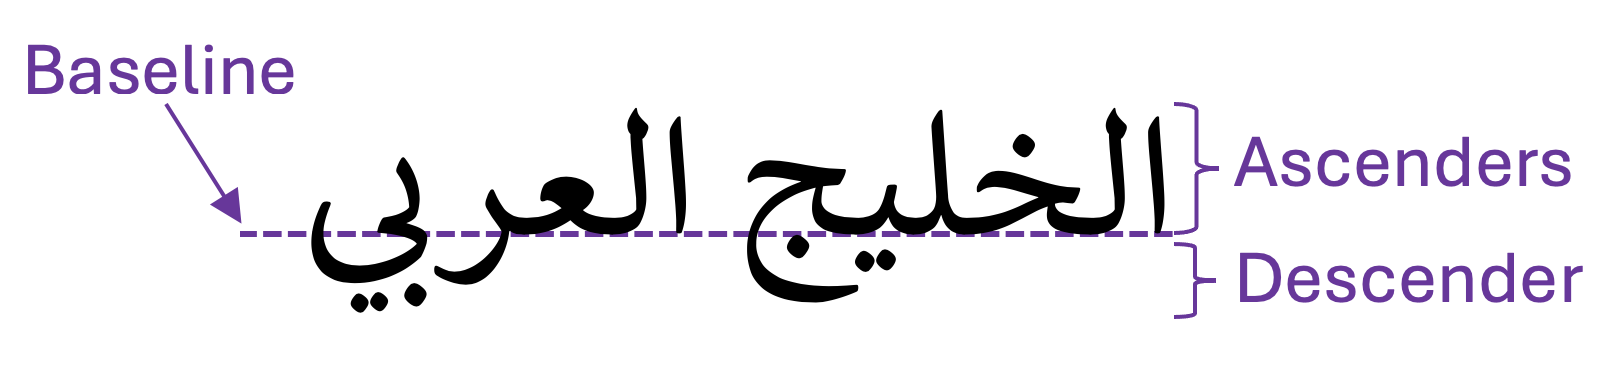
\includegraphics[width=0.8\linewidth]{Figs/fig2.png}
  \caption{some good caption.}
  \label{fig:ab}
\end{figure}

\subsubsection{Separating Characters and Word Segmentation}

Arabic includes six separating characters namely 
"\artext{ا}", "\artext{ر}", "\artext{ز}", "\artext{د}", "\artext{ذ}" and "\artext{و}", which are not connected to the characters that follow them. These separating characters divide words into smaller units known as Parts of Arabic Words (PAWs). Each word may consist of one or more PAWs depending on the presence of separating characters. Accurate segmentation of PAWs is critical for effective HTR, as it influences the ability to isolate and recognize individual characters within connected scripts. Examples of words composed of one, two, three, four, or five PAWs are presented in Table~\ref{table:words_with_paws}.

\begin{table}[ht]
  \renewcommand{\arraystretch}{1.3}
  \caption{Examples of Words with One, Two, Three, Four, and Five PAWs}
  \label{table:words_with_paws}
  \centering
  \begin{tabular}{|c|>{\centering\arraybackslash}p{2cm}|>{\centering\arraybackslash}p{3cm}|}
  \hline
  \textbf{No. of PAWs} & \textbf{Example} & \textbf{Division (Right-to-Left)} \\
  \hline
  \rule{0pt}{10pt} One PAW   & \artext{ليث}       & \artext{ليث} \rule[-8pt]{0pt}{8pt} \\ 
  \hline
  \rule{0pt}{10pt} Two PAWs  & \artext{حمزة}      & \artext{حمز  + ة} \rule[-8pt]{0pt}{8pt} \\ 
  \hline
  \rule{0pt}{10pt} Three PAWs & \artext{إبراهيم}  & \artext{إ + برا + هيم} \rule[-8pt]{0pt}{8pt} \\ 
  \hline
  \rule{0pt}{10pt} Four PAWs  & \artext{نورة}     & \artext{نو + رة} \rule[-8pt]{0pt}{8pt} \\ 
  \hline
  \rule{0pt}{10pt} Five PAWs  & \artext{أوراد}    & \artext{أ + و + را + د} \rule[-8pt]{0pt}{8pt} \\ 
  \hline
  \end{tabular}
\end{table}




\subsubsection{Overlapping in Handwritten PAWs}
In handwritten Arabic, PAWs may exhibit vertical overlapping, where characters within a word or between adjacent words overlap vertically. Figure ~\ref{fig:vo} illustrates examples of such overlapping, demonstrating how characters can intertwine, making segmentation and recognition more challenging. This overlapping is a common occurrence in cursive handwriting and requires robust HTR systems capable of accurately distinguishing and recognizing characters despite such distortions.

\begin{figure}[ht]
  \centering
  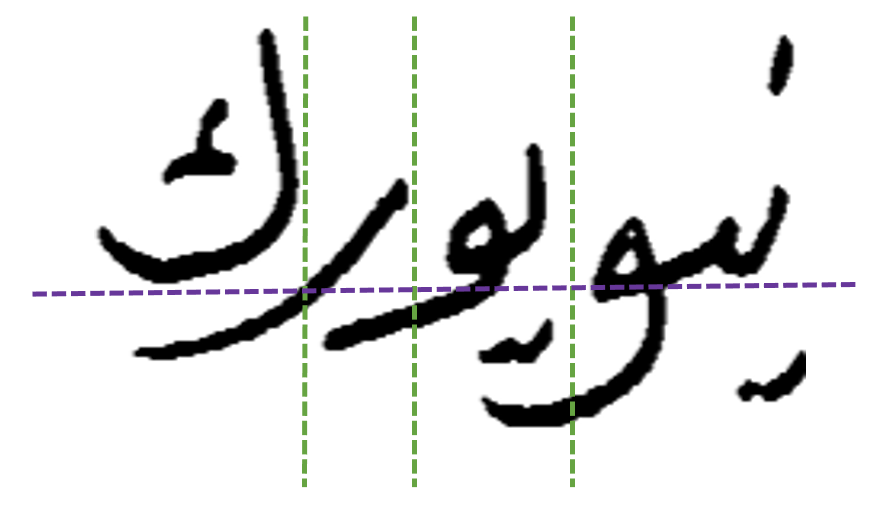
\includegraphics[width=0.7\linewidth]{Figs/fig3.png}
  \caption{Vertical Overlapping between 2 PAWs in the same word.}
  \label{fig:vo}
\end{figure}


\subsection{Challenges in Arabic HTR}

The recognition of Arabic handwritten text poses unique challenges due to the intricacies of the script, the variability of its handwritten forms, and the limitations of current resources and methodologies. This section explores these challenges in depth, highlighting the inherent difficulties that hinder the development of robust Arabic HTR systems.


\subsubsection{High Variability in Handwriting Styles}

Arabic handwriting exhibits a significant degree of variability, making it one of the most challenging scripts to process. Unlike many other scripts, Arabic handwriting allows for a broad range of stylistic diversity that is still considered acceptable. Individual differences in stroke thickness, letter spacing, slant, and elongation further contribute to the variation in handwritten forms. These stylistic differences are not arbitrary; they are often influenced by cultural and regional preferences. For example, traditional calligraphic styles such as "\artext{النسخ}" (Naskh), "\artext{الرقعة}" (Ruq’ah), and "\artext{الكوفي}" (Kufi) have distinct proportions and connections, which can manifest even in casual handwriting. Figure ~\ref{fig:mr}  illustrates examples of handwritten Arabic, showcasing the variability across different writers and styles.


\begin{figure}[ht]
  \centering
  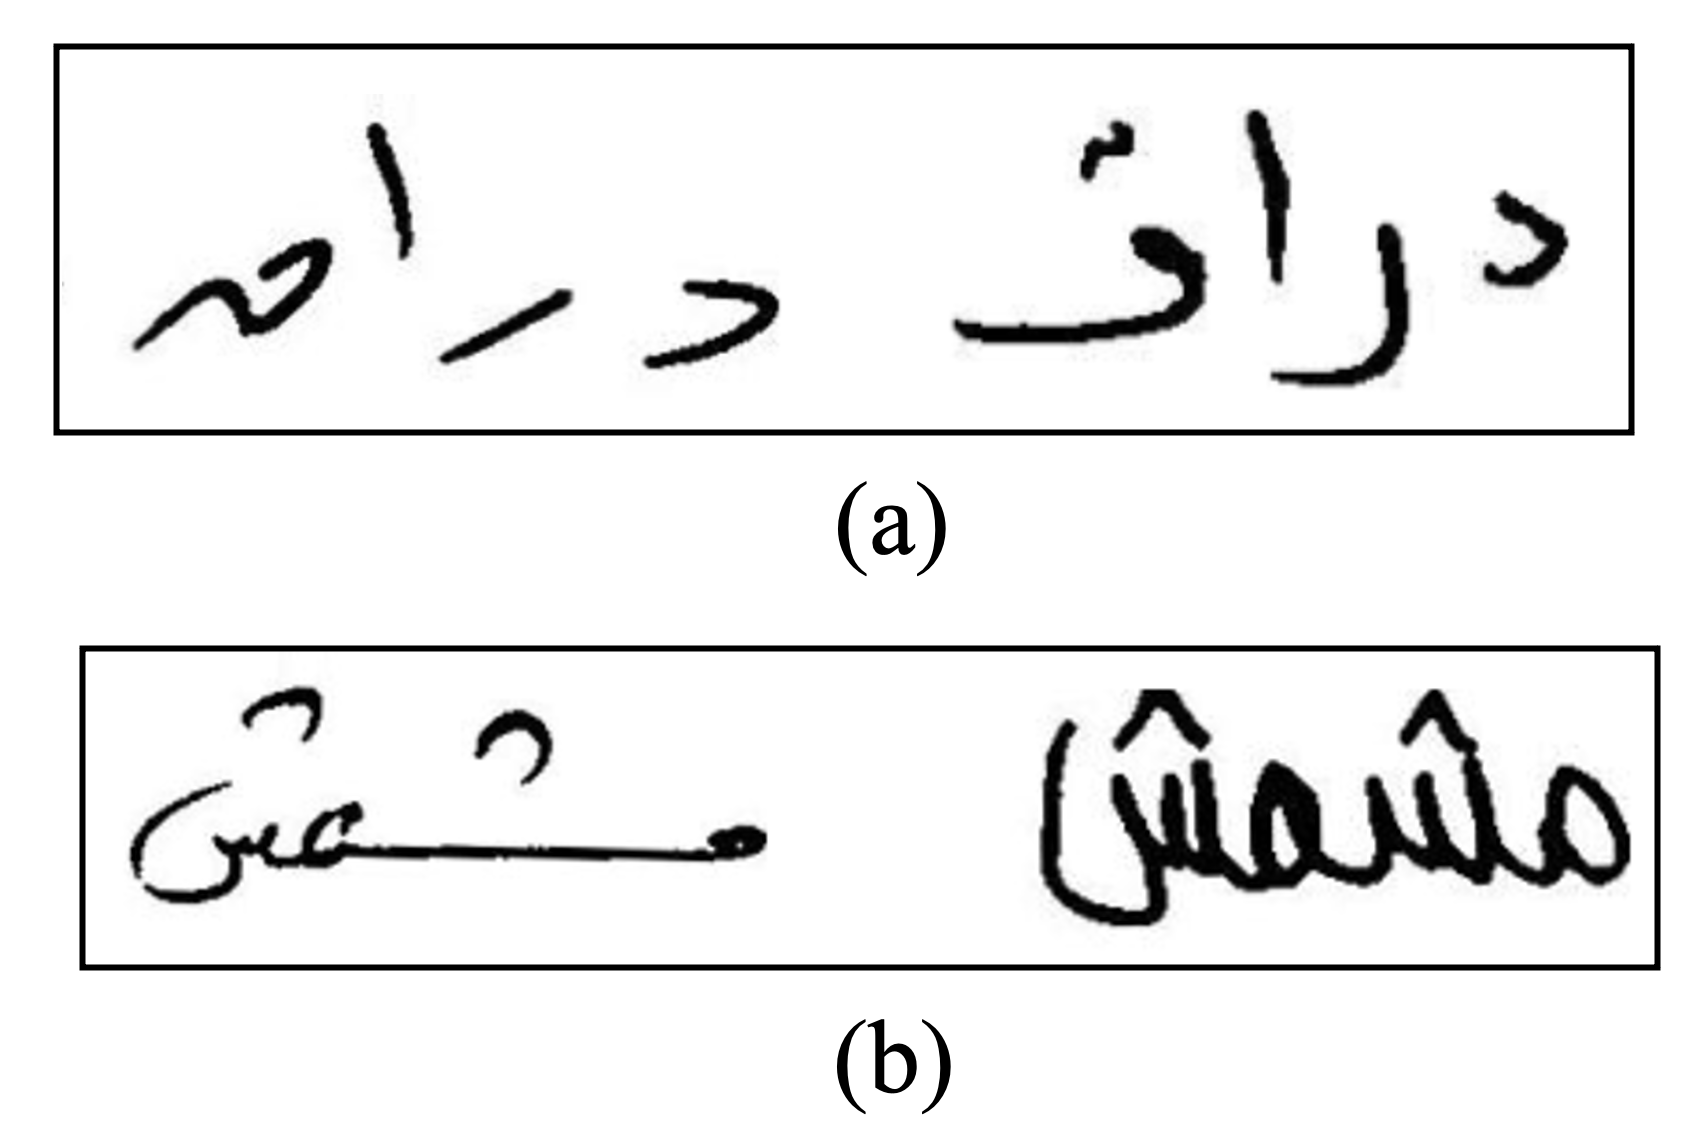
\includegraphics[width=0.7\linewidth]{Figs/fig4.png}
  \caption{Vertical Overlapping between 2 PAWs in the same word.}
  \label{fig:mr}
\end{figure}

Additionally, Arabic handwriting is not restricted to a single standardized form. Variants of Modern Standard Arabic (MSA) often appear in handwritten texts, including informal adaptations and regional orthographic practices. Although HTR systems are not tasked with interpreting dialects or regional meanings, the visual form of these handwritten variants—such as alternative spellings or elongated structures—introduces challenges in character recognition. This vast variability complicates segmentation and encoding, where traditional OCR systems fail due to their reliance on rigid, rule-based approaches. Unlike scripts with default spaces between characters, Arabic’s cursive nature creates continuous connections between letters, making segmentation into discrete units a formidable task. \\


///might end up removing, lets seee.


%%%%%%%%%NEED TO UN-GPT THIS%%%%%%%%%%

\subsubsection{Right-to-Left Directionality and Structural Bias}


The right-to-left (RTL) directionality of Arabic script introduces significant challenges for handwritten text recognition (HTR) systems, which are predominantly designed for left-to-right (LTR) languages. This fundamental difference impacts multiple aspects of HTR, including preprocessing, feature extraction, and sequence modeling, and requires specific adaptations to ensure that the system can effectively process Arabic text.

In Arabic, text begins at the top-right and flows toward the left, a structure that conflicts with the assumptions underlying most LTR-oriented algorithms. This discrepancy is particularly evident in preprocessing tasks, such as baseline detection and text alignment. For instance, the baseline of Arabic text is often affected by dynamic interactions between ascenders (e.g., "\artext{ط}") and descenders (e.g., "\artext{ي}"), which are more pronounced in cursive handwritten styles. Traditional baseline detection methods, which assume a uniform LTR structure, often misalign Arabic text, leading to errors in segmentation and recognition.


Convolutional Neural Networks (CNNs), a cornerstone of modern HTR systems, exacerbate these challenges with their sliding window mechanism. CNNs typically extract features by moving a kernel across the image from left to right. While effective for LTR scripts, this process introduces a structural bias when applied to Arabic text. Since Arabic handwriting flows from right to left, the CNN begins processing at the visual end of the word and progresses toward its beginning, disrupting the natural progression of contextual features. This mismatch results in suboptimal recognition of connected letters and diacritics, which are essential for accurate Arabic text recognition.

A commonly used workaround is to flip the input image horizontally, making the Arabic text visually appear as if it flows from left to right. While this enables LTR-designed systems to process the text more effectively, it introduces new challenges. Horizontal flipping can distort spatial relationships, particularly for diacritics or overlapping characters, and fails to address the inherent biases in the model architecture. For example, flipped input does not resolve issues in sequence alignment, where the reversed order may still impact downstream tasks like decoding.

In sequence modeling architectures, such as Recurrent Neural Networks (RNNs) and Transformers, RTL directionality creates additional challenges. RNNs, which process sequences step-by-step, are particularly sensitive to input order. A model trained on LTR text encounters Arabic text in reverse, handling the end of the sequence first and losing the natural semantic flow. Transformers, although more flexible due to their self-attention mechanisms, face similar problems. Positional encodings in pretrained Transformer models are often designed for LTR scripts, and their application to RTL text misaligns attention distributions, reducing the model’s ability to accurately weight the importance of characters at the beginning of words.

Addressing these biases requires architectural and algorithmic adaptations. For CNNs, designing RTL-compatible sliding window mechanisms that traverse the image in the correct direction aligns feature extraction with the natural flow of Arabic text. Similarly, retraining RNNs and Transformers with RTL-specific positional encodings or bidirectional capabilities helps to preserve the contextual integrity of Arabic handwriting. While preprocessing techniques such as horizontal flipping offer a temporary fix, they are insufficient for addressing the deeper structural challenges posed by RTL scripts. Robust adaptations at the model level are essential for achieving accurate and reliable recognition of Arabic handwritten text.


\subsubsection{Dataset Limitations}

The scarcity of high-quality, diverse datasets is one of the most significant obstacles to advancing Arabic HTR systems. While several datasets have been developed, such as KHATT and IFN/ENIT, they often fail to encompass the full spectrum of Arabic handwriting styles and scenarios. These datasets are typically limited in terms of writer demographics, regional variations, and text complexity. Moreover, many existing corpora focus exclusively on Modern Standard Arabic (MSA), excluding handwritten texts that exhibit informal, decorative, or application-specific features.

Another pressing issue is the size and annotation quality of available datasets. Compared to resources for widely studied languages like English, Arabic handwriting datasets are smaller in scale and less diverse. Annotated data for complex elements, such as diacritics, overlapping characters, or noisy inputs, remain particularly sparse. These deficiencies hinder the ability of HTR systems to generalize effectively across different writing styles and real-world applications. The creation of larger, more representative datasets with comprehensive annotations is essential for addressing these limitations and supporting the training of advanced HTR models.


%%%%%%%%%%%%%%%%%%%%%%%%%%%%%%%%%








\section{Related Work}
In this section, we review previous research on (), including traditional methods, advancements in deep learning, and the role of Arabic handwriting datasets in advancing the field.

Review of existing HTR systems for Arabic text.
Limitations of traditional feature-based approaches in HTR.
Advances in deep learning for handwriting recognition.
Datasets of Arabic Handwriting:
Overview of existing datasets: 
Introduction of the Muharaf dataset, its features, and its advantages.


\subsection{Preprocessing Techniques}

Preprocessing techniques are a crucial pre-requisite to any model's input. It ensures that the model is able to focus on the important features of the input to enable it to better detect patterns. In our case, our input is images that are handwritten Arabic documents and so it is crucial to ensure that the models are receiving input that can allow it to identify handwriting, letter styles, and strokes. 

A means of doing this is binarization. Binarization is a crucial preprocessing step that transfroms input images, whether they are RGB or grayscale, into a simplified binary format. The purpose of this is to highlight character strokes and remove unneccessary image color information. There are different ways to apply thresholds for binarization, the most prominent being global thresholding where beyond a certain threshold, the pixel is set to 1 and below that, set to 0. A more robust way is Otsu's method \cite{otsu1979aa} that finds an optimal global threshold by minimizing intra-class variance. It has been also proven to exhibit lower running times at a mean of 2 seconds \cite{sahlol2014proposed}. Another approach is differentiable binarization that integrates the binarization process into network training, allowing it to be part of optimization and loss calculations \cite{liao2022real}. Differentiable binarization uses an adaptive threshold map learned from the network to apply different thresholds on different parts of the image which is useful in areas of low confidence in boundary regions compared to areas of high confidence centrally within the image. Furthermore, this layer can be removed once the model is trained to ensure that inference time is not impacted.  

Another measure of preprocessing is noise removal. Noise removal is a crucial step as images often do not come in ideal conditions leading to poor model performance if fed directly. One of the techniques of noise removal is median filtering. The median of a group of pixels (3x3, 5x5, 7x7, etc.) that surround a specific pixel (its neighborhood) replaces the pixel to smooth out and reduce noise within the image \cite{sahlol2014proposed,alghyaline2023arabic}. Another common category of techniques is morphological operations. These operations manipulate the shape of the input images. These operations include dilation, erosion, opening, and closing \cite{alghyaline2023arabic}. Dilation adds pixels to the boundaries of objects in an image making them thicker within the image. Conversely, erosion removes pixels from object boundaries, eliminating pixels that are isolated. Opening and closing are then combinations of erosion and dilation that help find the right balance between refining object shapes and eliminating noise. 




\subsection{Deep Learning Methods for OCR}





\subsection{Datasets of Arabic Handwriting}

Several datasets have been developed for Arabic handwriting research, (). These datasets differ in focus, size, and availability. Below, we summarize the most relevant ones including WAHD, KHATT, Balamand, and Muharaf.



AHTID/MW .. IFN/ENIT,, MADCAT
Arabic Handwritten Text Images Database written by Multiple Writers (AHTID/MW) dataset




\begin{itemize}
  
    \item \textbf{KHATT Dataset \cite{mahmoud2014khatt}:} \\ 
    The KHATT dataset is a modern Arabic handwriting dataset comprising 4,000 paragraphs written by 1,000 scribes, with six paragraphs contributed by each.  was developed jointly by researchers from KFUPM (Saudi Arabia), TU Dortmund (Germany), and TU Braunschweig (Germany). 



    \item \textbf{IFN/ENIT Dataser \cite{mahmoud2014khatt}:} \\
    Most cited database. Contains 26,459 handwriting samples


    \item \textbf{Muharaf Dataset \cite{saeed2024muharaf}:} \\
    The Muharaf dataset, used in this study, is the largest publicly available Arabic dataset with fully annotated and transcribed historical manuscripts at the text-line level. It includes 1,644 pages (1,216 public and 428 restricted), spanning the early 19th to the early 21st century, with 36,311 text lines (24,495 public). Line-level images, stored in PNG format, were generated using line warping software to create consistent horizontal grids, and extensive metadata is provided in JSON format.
  
\end{itemize}


\section{Methodology}



\subsection{Data Preparation and Preprocessing}

% The KHATT dataset was unaccessable (webside was corrupted), we could not find the official source. we find differnet versions online e.g. kaggle and huggingface. we ededup seleetign this one to use. although it does not have all the # of lines reported in other papers. so we used the one from kaggle. this was was already made into lines and preprocessed (as far as we could tell) with ground truth lables in txt format

To prepare the data for model training, we utilized the filtered line-by-line images of the KHATT dataset from *CITE KAGGLE LINK HERE*. The data has already been preprocessed by binarizing the images, cropping out the unnecessary whitespaces around the handwritten texts, and straightening out the lines as much as possible. Thus, the only preprocessing we had to do was adhering to the paper's *CITE THE PAPER WE ARE REPRODUCING HERE* resizing of the images to 64 pixels for the height and 1048 for the width, normalizing the images, and horizontally flipping the images and the labels because a CNN traverses the image from left-to-right. Furthermore, we used a 70-15-15 train-validation-test split stratified on the length of the sentences because longer sentences may impact the discriminative ability of the model. Before this step, we had to aggregate sentences with less than eight characters to ensure an adequate number of samples of varying sentence lengths for each split. Lastly, we did not employ data augmentations because when they were introduced, the model stopped learning after some epochs.

\subsection{Supervised Learning}

\subsubsection{Model Architecture}

As we aim to reproduce the results of *CITE PAPER WE ARE REPRODUCING*, we reimplemented the architecture detailed in the paper to the best of our ability. This led to us creating the CNN-BiLSTM architecture, which is the most popular framework for the OCR task *CITE PAPERS THAT USED CNN-BiLSTMs* for a number of reasons. Moving away from using handcrafted features like SIFT descriptors, the CNN is responsible for extracting the hierarchical spatial features inherent in an image, especially in handwritten text images. As the CNN traverses the handwritten text from left-to-right, it learns, through its various filters, how to capture the the shapes of diacritics, letters, and words in Arabic handwritten text. Adding more and more layers can result in a better representation of the handwritten text. However, training deeper networks is not necessarily easy, mostly due to the vanishing gradient problem -- where multiplying many small gradients together will result in hindering the neural network's learning process. Thus, the introduction of skip connecions or residual connections.

Skip connections allows a layer to bypass one or more subsequent layers by adding or concatenating its output as another input to a non-consecutive layer. That is, they allow the outputs of a layer to be fed to a much later layer. This is the foundational idea of the ResNet architecture. With these skip connections, training deeper networks is easier and the impact of vanishing gradients is reduced. We recreated the ResNet32 architecture, serving as the backbone and the feature extractor of our handwritten text images. The only change we made was adding a \( 1 \times 1 \) convolutional layer in the residual block to handle the varying filter sizes for the skip connections. After adding a dropout layer after the ResNet block to lessen the chances of overfitting to the training set, the feature maps are fed into the three BiLSTMs. The three BiLSTMs deal with the sequential nature of handwriting and the necessity in considering the connections between each letter to form a word, especially important in cursive-styled text like Arabic. Succeeding the dropout layer directly after all three BiLSTM layers is a fully connected dense layer with CTC as the loss function to help optimize how the model learns how to align its prediction to the groundtruth labels. Both dropout layers randomly drop neurons at a rate of 0.2 and we added batch normalization layers in the residual blocks for training stabilization and faster convergence.

\subsubsection{Model Training and Evaluation}

OCR is a sequence-to-sequence problem because a sequence of characters are recognized from the images and a sequence of characters are predicted to match the characters seen from the handwritten text. For this specific task, we used the CTC as our loss function during our training process, lasting 300 epochs. The Adadelta optimizer was used with an initially high learning rate of 1.0. The hyperparameters for model training are mentioned below:

We used various callbacks to help the model not get stuck in a local minimum and to boost generalization capabilities. The two main callbacks for these goals are ReduceLROnPlateau and EarlyStopping. ReduceLROnPlateau is a scheduler that adaptively reduces the learning rate whenever the validation loss plateaus for every 5 epochs. The reduction in the learning rate is by a factor of 0.5 to ensure smoother network convergence. The learning rate scheduler's parameters are detailed in *TABLE HERE*. To prevent wasting time and resources on overtraining and to avoid overfitting, EarlyStopping with a patience of 50 epochs is used. If the model does not improve on the evaluation metric monitored by EarlyStopping -- validation loss in our case -- then, model training will be halted.

To supplement the training process, we utilized additional callback functions. We periodically saved the model every 25 epochs, outputted training and validation metrics for each epoch, and cleared the displayed outputs in the Jupyter Notebook every 10 epochs to improve the readability of the notebook during model training.

Due to the nature of this task, especially with complex scripts such as Arabic, we had to resort to robust metrics to evaluate the performance of the model. These are character error rate (CER) and word error rate (WER). CER measures the character-level differences between the predicted text and the groundtruth, while WER is concerned about word-level discrepancies. These particular metrics are derived from calculating the Levenshtein distance, a meaure of how different is a sequence of characters from another. The Levenshtein Distance is the minimum number of transformations necessary to convert a sequence into another sequence. These sequences could be insertions, deletions, or substitutions. Below are the similar mathematical formulations for CER and WER:

Model training was conducted on two NVIDIA A100 (SXM4) Tensor Core GPUs, each with 80 GB of memory. One was provided by the American University of Sharjah's (AUS) Computer Science and Engineering (CSE) Department from their Artificial Intelligence (AI) lab, while another was accessed remotely through RunPod's platform.

\[
    \text{CER} = \frac{S + D + I}{N}
\]

\begin{itemize}
  \item \( S \) = Number of character substitutions
  \item \( D \) = Number of character deletions
  \item \( I \) = Number of character insertions
  \item \( N \) = Total number of characters in the reference (ground truth)
\end{itemize}

\[
    \text{WER} = \frac{S + D + I}{N}
\]

\begin{itemize}
  \item \( S \) = Number of word substitutions
  \item \( D \) = Number of word deletions
  \item \( I \) = Number of word insertions
  \item \( N \) = Total number of words in the reference (ground truth)
\end{itemize}


\section{Results and Discussion}

\blindtext[2]

\section{Conclusions and Future Work}

\blindtext[3]




 
% Bibliography section
\bibliographystyle{IEEEtran}  % IEEE style
\bibliography{references}

\end{document}